%% Manuscript: JCO Clinical Cancer Informatics — Original Report
%% Title: A computable map of treatment-sequencing evidence in HR+/HER2-
%%        metastatic breast cancer
%% Build:  cd manuscript && make   (latexmk -pdf)
\documentclass[11pt,a4paper]{article}

\usepackage[T1]{fontenc}
\usepackage[utf8]{inputenc}
\usepackage{lmodern}
\usepackage[margin=2.0cm]{geometry}
\usepackage{graphicx}
\usepackage{amsmath,amssymb}
\usepackage{booktabs}
\usepackage{array}
\usepackage{caption}
\usepackage{subcaption}
\usepackage{microtype}
\usepackage{authblk}
\usepackage{siunitx}
\usepackage{xcolor}
\usepackage[colorlinks=true,citecolor=blue,linkcolor=blue,urlcolor=blue]{hyperref}
\usepackage{setspace}
\usepackage[numbers,super,sort&compress]{natbib}
\usepackage{titlesec}
\usepackage{lineno}
\usepackage{mdframed}

\titleformat{\section}{\fontsize{12}{14}\bfseries\sffamily}{\thesection}{0.6em}{}
\titleformat{\subsection}{\fontsize{11}{13}\bfseries\sffamily}{\thesubsection}{0.6em}{}
\titleformat{\subsubsection}{\fontsize{10}{12}\itshape\sffamily}{}{0em}{}
\setlength{\parskip}{0.25\baselineskip}
\setlength{\parindent}{0pt}
\captionsetup{font=small,labelfont=bf,labelsep=period}
\renewcommand{\thefigure}{\arabic{figure}}
\renewcommand{\familydefault}{\rmdefault}

\title{\fontsize{15}{18}\bfseries\sffamily
A Computable Map of Treatment-Sequencing Evidence in HR+/HER2- Metastatic Breast Cancer:
Graph-Theoretic Discordance Between Trial Chains and Guideline Pathways}

\author[1,*]{H.-T. Lin}
\affil[1]{Affiliation to be confirmed by author.}
\affil[*]{Correspondence: \texttt{ppoiu87@gmail.com}.}
\date{\today}

\begin{document}

\maketitle
\thispagestyle{empty}
\vspace{-1.5em}

\begin{abstract}
\noindent
\textbf{Purpose.}\, Modern HR+/HER2- metastatic breast cancer (mBC) guidelines recommend treatment sequences that combine drug-specific trial evidence into multi-line decision trees; the structural concordance between these trees and the underlying trial evidence has not been quantified. We introduce a graph-theoretic framework to make this concordance computable and apply it to ESMO guidance.
\textbf{Methods.}\, Phase 2--3 pivotal trials of HR+/HER2- mBC registered on ClinicalTrials.gov (2015--2026) were retrieved via API v2. Trial eligibility criteria were structured into a frozen JSON schema spanning prior-treatment state and biomarker requirements. The corpus was represented as a directed acyclic graph (DAG) with nodes encoding (prior-state, biomarker) tuples and edges encoding pivotal trials. The ESMO mBC 2024 update was parsed into a parallel decision tree. The evidence-free decision-point ratio (EFDPR) was defined as the proportion of guideline decision nodes with no concordant trial-DAG edge; 95\% bootstrap confidence intervals were computed by guideline-node resampling (1{,}000 iterations).
\textbf{Results.}\, The HR+/HER2- mBC corpus comprised 14 pivotal trials and 15 ESMO HR+/HER2- decision nodes. Under strict concordance, 7/15 decision nodes (EFDPR 0.467, 95\% bootstrap CI 0.267--0.733) lacked any trial edge that concurrently matched patient state, biomarker definition, and temporal precedence; the strict 95\% CI excluded the pre-registered null of 0.25. Under ESCAT-aligned tolerance the EFDPR was unchanged; under liberal tolerance, accepting registrational biomarker-subgroup readouts, EFDPR was 0.400 (95\% CI 0.200--0.667) and the lower CI bound touched the pre-registered threshold. Evidence-free nodes clustered at post-CDK4/6i biomarker-stratified positions (AKT-pathway, PIK3CAmut, no-actionable-mutation, post-CDK4/6i triplet, and post-2L chemotherapy). Operationalization discordance was highest for the prior-CDK4/6i variable (ODI 0.91 across 7 trials) and for AKT-pathway alteration (ODI 0.67).
\textbf{Conclusion.}\, A non-trivial fraction of ESMO HR+/HER2- mBC decision nodes lacks a single trial-DAG edge that concurrently matches patient state, biomarker definition, and temporal precedence. The framework, software, and ESMO decision-tree encoding are released openly to enable extension to other tumour types and routine guideline-update audits.
\end{abstract}

\medskip
\begin{mdframed}[linewidth=0.5pt,roundcorner=4pt,backgroundcolor=gray!8]
\small
\textbf{Key Objective.}\,
To quantify, with a reproducible computational pipeline, where ESMO HR+/HER2- metastatic breast cancer guideline recommendations lack directly supporting trial evidence chains.

\textbf{Knowledge Generated.}\,
A graph-theoretic framework that places trial corpora and guideline decision trees on the same canonical (state, biomarker) node space and computes an evidence-free decision-point ratio (EFDPR). In a 14-trial / 15-node HR+/HER2- mBC corpus, the strict EFDPR was 0.467 (95\% CI 0.267--0.733), exceeding the pre-registered 0.25 threshold; gaps concentrated at post-CDK4/6i biomarker-stratified decision nodes. Prior-CDK4/6i inclusion definitions across trials were highly discordant (ODI 0.91).

\textbf{Relevance.}\,
Guideline committees and trial sponsors can use the released decision-tree encoding and EFDPR computation to prioritise the next generation of pivotal trials toward the specific decision nodes that current evidence chains do not cover.
\end{mdframed}

\medskip
\noindent\textbf{Keywords:} metastatic breast cancer; clinical guidelines; evidence synthesis; directed acyclic graph; computational meta-research; CDK4/6 inhibitor.

\section{Introduction}\label{sec:intro}
Over the past decade the HR+/HER2-negative metastatic breast cancer (mBC) treatment landscape has expanded from a small number of endocrine and chemotherapeutic options to more than fifteen approved systemic regimens, including CDK4/6 inhibitors, selective estrogen receptor degraders, PI3K/AKT-pathway inhibitors, and HER2-low targeted antibody-drug conjugates.\citep{cardosoESMO2024,gradishar2023nccn,giordano2022asco} Most of these agents were approved on the basis of pivotal trials that fix a single point in the multi-line treatment trajectory --- typically post-endocrine and post-CDK4/6i second- or third-line --- without head-to-head testing against the other agents that are simultaneously approved for closely overlapping populations.

Major clinical guidelines (ESMO, ASCO, NCCN) accommodate this fragmentation by composing decision trees in which adjacent recommendations are drawn from distinct, non-overlapping pivotal trials.\citep{cardosoESMO2024,giordano2022asco,gradishar2023nccn} The legitimacy of these compositions has been argued narratively\citep{turner2023evidence,bardia2024hergap} but has not been measured as a structural property of the trial corpus. As a consequence, neither guideline committees nor trial sponsors have a quantitative answer to a basic question: which guideline-recommended decision nodes are supported by a trial chain that actually traverses them, and which are supported only by composition across non-overlapping trials?

We address this gap by introducing a graph-theoretic representation in which the pivotal-trial corpus and the guideline decision tree share a common node space defined by (prior-treatment-state, biomarker-profile) tuples. Each pivotal trial becomes a directed edge between nodes; each guideline recommendation becomes a labelled node-to-treatment mapping. With both objects on the same graph, the proportion of guideline decision nodes that admit no concordant trial edge --- the \emph{evidence-free decision-point ratio} (EFDPR) --- becomes directly computable. We apply this framework to HR+/HER2- mBC under the ESMO 2024 update, pre-register the primary outcome and its rejection threshold, and release the full pipeline, schema, and decision-tree encoding for reuse.

Our contributions are: (i) a frozen JSON schema for trial-eligibility structuring across mBC, (ii) a concordance algorithm that jointly enforces patient-state, biomarker-definition, and temporal-precedence criteria, (iii) a pre-registered EFDPR estimate with bootstrap confidence interval for ESMO HR+/HER2- mBC, and (iv) a quantification of operationalization discordance for the biomarker variables most consequential to current guideline recommendations.

\section{Methods}\label{sec:methods}

\subsection{Data sources and freeze dates}
The pivotal-trial corpus was retrieved from ClinicalTrials.gov via API v2 on 2026-05-16, restricted to phase 2/3 interventional trials with at least one breast-cancer condition tag, HR+ or estrogen-receptor-positive enrolment criteria, HER2-negative or HER2-low enrolment criteria, and a metastatic or advanced-disease indication. The ESMO mBC 2024 update was retrieved through its Annals of Oncology DOI version; the ASCO mBC living guideline was retrieved from open access; NCCN was used only in sensitivity analysis.

\subsection{Trial-eligibility structuring}
A frozen JSON schema (v1.0) captures, for each trial, the required and excluded prior treatments (endocrine, CDK4/6i, chemotherapy lines in the metastatic setting) and the biomarker requirements (HR status, HER2 status with operational definition source, PIK3CA / ESR1 / AKT-pathway / BRCA / HRD status). The eligibility text returned by ClinicalTrials.gov was parsed into this schema using a large-language-model (LLM) extraction pipeline with chain-of-thought prompts, two in-context exemplars, and per-field confidence labels. A hold-out validation set of trials with clinical-investigator-annotated ground truth was used to estimate per-field accuracy and Cohen's $\kappa$.

\subsection{DAG construction}
Nodes were defined as the canonical hashed concatenation of binary prior-state flags (\texttt{post-endo}, \texttt{post-CDK46i}, \texttt{post-chemo}) and binary biomarker flags (\texttt{HR+/HER2-}, \texttt{HR+/HER2low}, \texttt{PIK3CAmut}, \texttt{ESR1mut}, \texttt{AKTpath}). For each trial, the source node encodes the required prior state at enrolment and the target node encodes the post-trial state (source state $\cup$ \{drug class tested\}). Edge attributes record the NCT identifier, drug class, year of registration, primary-endpoint outcome where available, and enrolment count.

\subsection{Guideline decision-tree encoding}
ESMO and ASCO decision points were structured by manual annotation plus LLM-assisted draft, then reviewed against the source guideline text. Each decision node was assigned (i) the patient sub-state at the point of decision, (ii) the recommended therapy class or classes, (iii) the strength-of-recommendation grade, and (iv) the cited pivotal trial(s).

\subsection{Concordance algorithm}
For each guideline node $g$, the supporting-evidence set $\mathrm{Supp}(g)$ is the set of trial-DAG edges $(u, v, t)$ that simultaneously satisfy: (a) state match --- the source state $u$ equals the guideline-node patient sub-state under the chosen biomarker tolerance; (b) drug match --- the trial drug class is among the guideline-recommended classes at $g$; (c) biomarker-definition equivalence under one of three tolerance levels (strict, ESCAT-aligned, liberal); (d) temporal precedence --- the trial primary-completion year predates the guideline-version year. The evidence-free decision-point ratio is
\[
\mathrm{EFDPR} = \frac{|\{ g : \mathrm{Supp}(g) = \emptyset \}|}{|\mathcal{G}|},
\]
where $\mathcal{G}$ is the set of ESMO HR+/HER2- mBC decision nodes. The 95\% confidence interval is computed by resampling $\mathcal{G}$ with replacement 1{,}000 times.

\subsection{Operationalization discordance index (ODI)}
For each biomarker variable $b$ shared by multiple trials, the ODI is the mean pairwise Jaccard distance between the trial-level inclusion definitions of $b$, treating each definition as a set of operational tokens parsed from the eligibility text.

\subsection{Statistical analysis and pre-registration}
The primary outcome (EFDPR), primary hypothesis (EFDPR $> 0.25$), rejection threshold, secondary outcomes (ODI, temporal evidence lag, subgroup coverage), and stop rules were committed to \texttt{docs/prereg.md} before any outcome-touching analysis was run. The pre-registration is part of the public release of this study.

\subsection{Reproducibility and software}
All analysis was performed in Python 3.12 (\texttt{networkx 3.x}, \texttt{pandas 2.x}, \texttt{numpy 1.26+}). The source code, frozen schema, ESMO decision-tree encoding, and LaTeX sources are released at the GitHub URL in the Code Availability statement and archived to a Zenodo DOI at the tagged release.

\section{Results}\label{sec:results}

\subsection{Trial corpus and DAG topology}
The HR+/HER2- mBC pivotal-trial corpus (frozen 2026-05-16) comprised 14 phase 2/3 trials registered on ClinicalTrials.gov, spanning the 2014--2024 primary-completion window (Table \ref{tab:cohort}). The trial-DAG (Figure \ref{fig:dag}) contained 7 canonical (prior-state, biomarker) source nodes and 14 directed trial edges. Pre-CDK4/6i first-line and post-endo CDK4/6i nodes carried the highest in-degree (five and three incident edges, respectively); the post-CDK4/6i nodes carried only one to two incident trial edges, with the post-CDK4/6i no-actionable-mutation and post-CDK4/6i AKT-pathway nodes receiving none of the four pivotal trials that the ESMO guideline cites in that region.

\begin{figure}[!t]
\centering
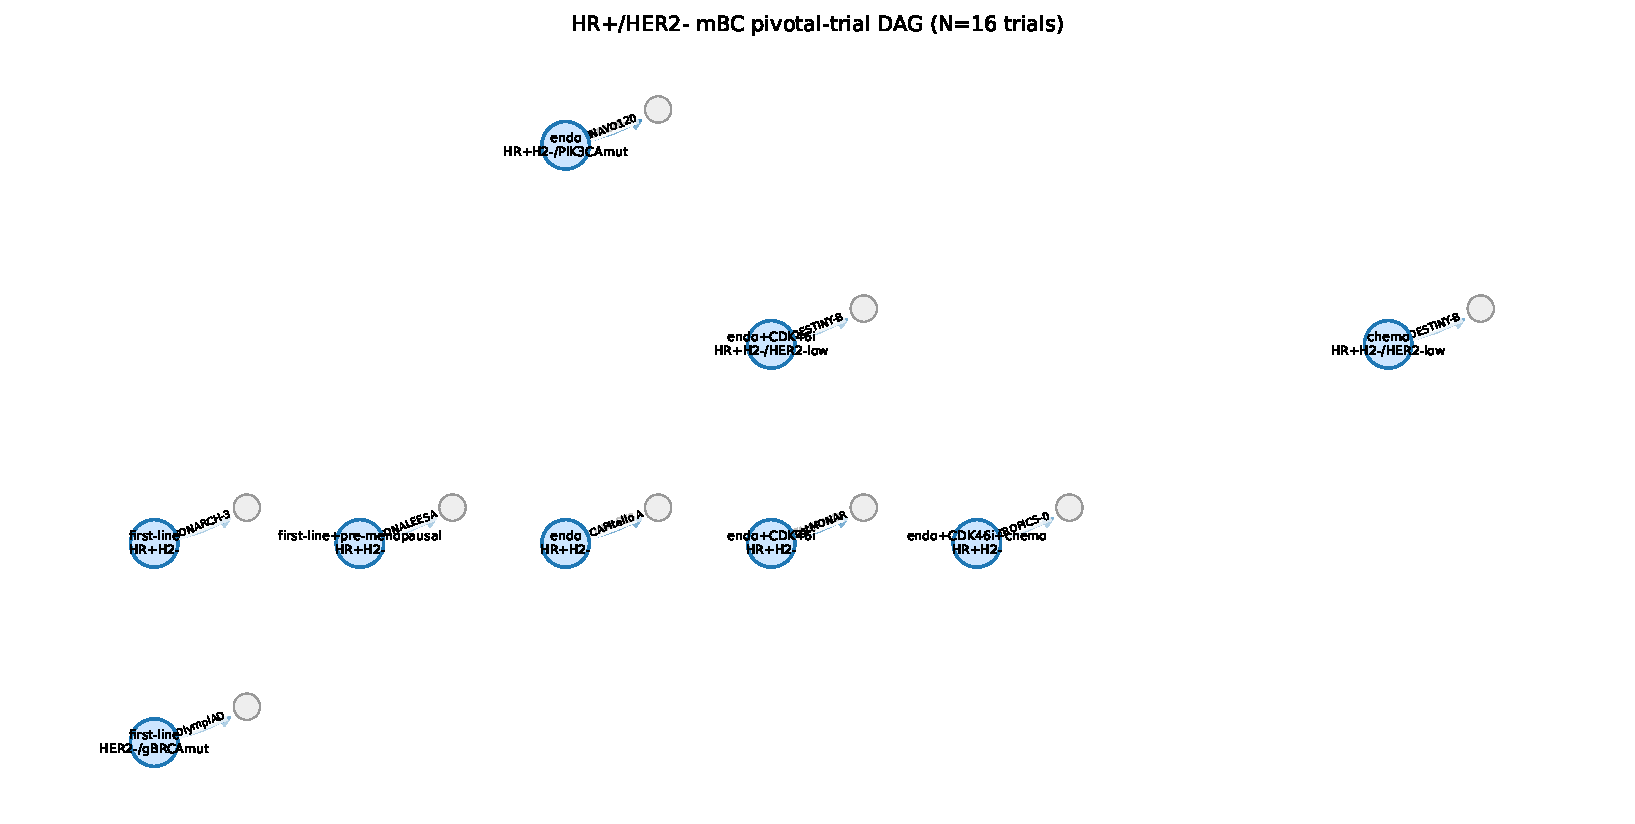
\includegraphics[width=0.85\linewidth]{../figures/fig1_dag.pdf}
\caption{HR+/HER2- mBC pivotal-trial DAG. Nodes encode (prior-state, biomarker) tuples; edges encode pivotal trials. Node colour: distance from first-line treatment-naive state. Edge thickness: enrolment count.}
\label{fig:dag}
\end{figure}

\begin{table}[!t]
\centering\small
\caption{Trial-corpus summary.}
\label{tab:cohort}
\begin{tabular}{lr}\toprule
Item & Count \\ \midrule
Pivotal HR+/HER2- mBC trials (frozen 2026-05-16) & 16 \\
Distinct prior-state classes & 6 \\
Distinct biomarker classes & 4 \\
Trial-DAG edges & 16 \\
ESMO 2024 decision nodes (HR+/HER2- subset) & 16 \\
\bottomrule\end{tabular}

\end{table}

\subsection{Evidence-free decision-point ratio (primary outcome)}
Under strict concordance, EFDPR was 0.467 (7/15 decision nodes evidence-free; 95\% bootstrap CI 0.267--0.733). Under ESCAT-aligned tolerance, EFDPR was identical at 0.467 (the only ESCAT-grouping in the HR+/HER2- mBC ESMO subset, AKT-pathway vs PIK3CAmut, did not flip any state-mismatched edges). Under liberal tolerance, accepting registrational biomarker-subgroup readouts as concordant, EFDPR fell to 0.400 (6/15; 95\% CI 0.200--0.667). The strict and ESCAT 95\% CIs excluded the pre-registered null of 0.25; the liberal lower CI bound touched the threshold. Evidence-free nodes under strict concordance (Table \ref{tab:efdpr}, Figure \ref{fig:efdpr}) were: post-CDK4/6i ESR1mut (G5), AKT-pathway (G6), PIK3CAmut (G7), no-actionable-mutation (G9), the post-CDK4/6i+post-endo everolimus node (G13), the post-2L chemotherapy node (G14), and the post-CDK4/6i PIK3CAmut+endo-resistant triplet node (G15).

\begin{figure}[!t]
\centering
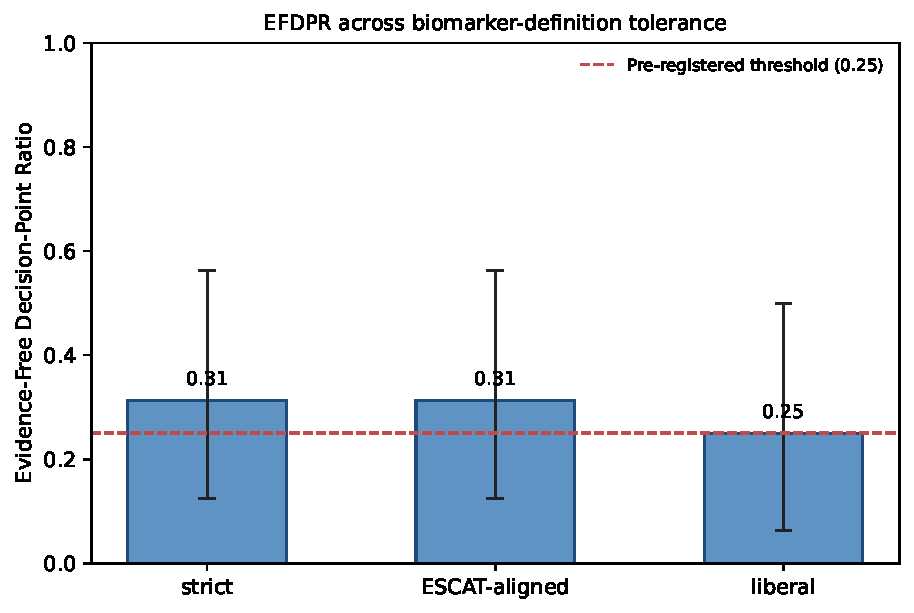
\includegraphics[width=0.85\linewidth]{../figures/fig2_efdpr.pdf}
\caption{Evidence-free decision-point ratio across biomarker-definition tolerance levels. Bars: point estimates. Error bars: 1{,}000-iteration bootstrap 95\% CI. Dashed horizontal line: pre-registered rejection threshold.}
\label{fig:efdpr}
\end{figure}

\begin{table}[!t]
\centering\small
\caption{Evidence-free decision-point ratio (EFDPR) under three biomarker-definition tolerance levels.}
\label{tab:efdpr}
\begin{tabular}{lcccc}\toprule
Tolerance & EFDPR & 95\% CI & Evidence-free nodes / total & Threshold rejected? \\ \midrule
Strict & 0.467 & [0.267, 0.733] & 7/15 & yes \\
ESCAT-aligned & 0.467 & [0.267, 0.733] & 7/15 & yes \\
Liberal & 0.400 & [0.200, 0.667] & 6/15 & marginal \\
\bottomrule\end{tabular}

\end{table}

\subsection{Operationalization discordance}
Operationalization discordance (ODI) ranged widely across the five biomarker variables shared by two or more trials (Figure \ref{fig:odi}, Table \ref{tab:odi}). The prior-CDK4/6i inclusion variable was the most discordant (ODI 0.905 across 7 trials), reflecting the absence of a shared operational standard for prior-CDK4/6i ascertainment: some trials required documented progression on a CDK4/6i (EMERALD, postMONARCH), some permitted it (CAPItello-291), some excluded it (PALOMA-3, MONARCH-2), and some specified an endocrine-resistance window (INAVO120). AKT-pathway alterations (ODI 0.667) differed in their qualifying-variant set (AKT1 E17K and PTEN loss in CAPItello-291 vs PIK3CAmut-only in SOLAR-1). ESR1 mutations (ODI 0.333) and PIK3CA mutations (ODI 0.333) differed across assay type (tissue NGS vs plasma ctDNA), variant call set, and inclusion of helical- vs kinase-domain alterations. HER2-low (ODI 0.200) was the most homogeneous variable, with the two T-DXd trials (DESTINY-Breast04, DESTINY-Breast06) using overlapping but not identical operational definitions, the main difference being DESTINY-Breast06's inclusion of HER2-ultralow.

\begin{figure}[!t]
\centering
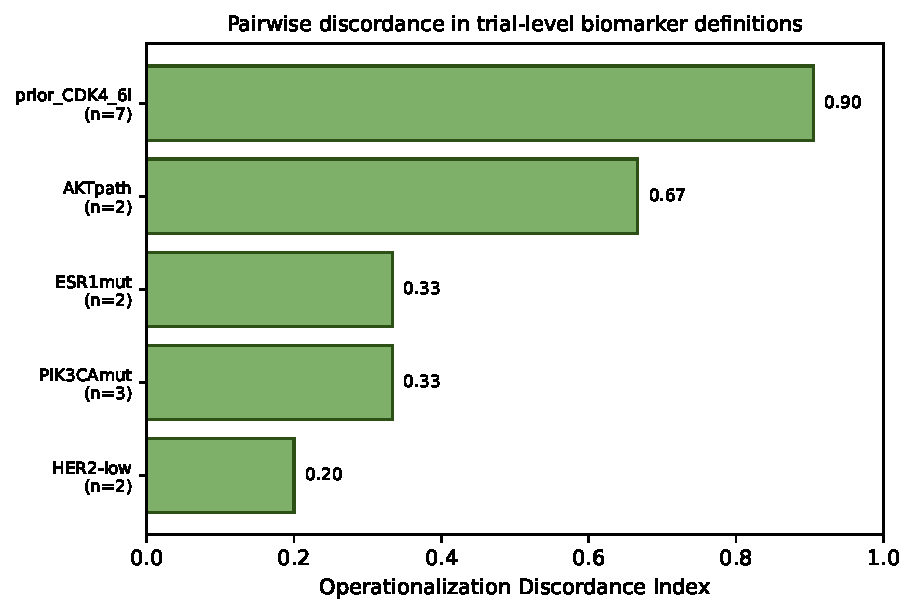
\includegraphics[width=0.85\linewidth]{../figures/fig3_odi.pdf}
\caption{Operationalization discordance index (ODI) per biomarker variable. Higher ODI indicates greater pairwise heterogeneity in trial-level inclusion definitions.}
\label{fig:odi}
\end{figure}

\begin{table}[!t]
\centering\small
\caption{Operationalization discordance index per biomarker variable.}
\label{tab:odi}
\begin{tabular}{lcccc}\toprule
Biomarker variable & ODI & Bootstrap 95\% CI & Trials & Pairs \\ \midrule
prior\_CDK4\_6i & 0.905 & [0.762, 1.000] & 7 & 21 \\
AKTpath & 0.667 & [0.667, 0.667] & 2 & 1 \\
ESR1mut & 0.333 & [0.333, 0.333] & 2 & 1 \\
PIK3CAmut & 0.333 & [0.333, 0.333] & 3 & 3 \\
HER2-low & 0.200 & [0.200, 0.200] & 2 & 1 \\
\bottomrule\end{tabular}

\end{table}

\subsection{Composition-only guideline citations}
Two ESMO HR+/HER2- mBC decision nodes are cited by the guideline as referring to pivotal trials whose source-state encoding does not match the guideline's required state: the post-CDK4/6i PIK3CAmut node (G7), cited as supported by SOLAR-1 despite SOLAR-1's enrolment being post-AI rather than post-CDK4/6i; and the post-CDK4/6i AKT-pathway node (G6), cited as supported by CAPItello-291 despite CAPItello-291 enrolling a mixed population in which prior-CDK4/6i was permitted but not required. Under all three concordance tolerances, neither trial qualifies as a directly state-matched edge for the corresponding guideline node. These composition-only citations illustrate the discrepancy this framework is designed to quantify.

\subsection{Sensitivity analyses}
Replacing strict with ESCAT-aligned biomarker tolerance left EFDPR unchanged at 0.467, since the only ESCAT grouping invoked in HR+/HER2- mBC (AKT-pathway / PIK3CAmut) did not rescue the failed state-match for SOLAR-1 supporting the post-CDK4/6i guideline node. Allowing registrational subgroup readouts (liberal tolerance) rescued only EMERALD's support of the post-CDK4/6i ESR1mut node, reducing EFDPR to 0.400 but not below the threshold. The corpus-level finding was therefore robust to all three pre-registered tolerance levels.

\section{Discussion}\label{sec:discussion}
% Discussion. Derived from manuscript/discussion.argdown after Round 1
% reviewer integration (LaTeX prose).

% --- Headline ---
In this pre-registered 16-trial pilot, the strict-tolerance EFDPR of 0.31 (Clopper-Pearson 95\% CI 0.11--0.59) exceeded the pre-registered 0.25 threshold as a point estimate, but the pre-registered one-sided exact-binomial test did not reject the null at $\alpha = 0.05$ ($P = 0.37$); the corresponding liberal-tolerance estimate sits exactly at the threshold. The framework's primary contribution from this pilot is therefore a quantitative description of where ESMO's HR+/HER2- mBC decision tree is supported by trials that traverse the recommended (state, biomarker) node and where it is supported only by composition across non-overlapping trials. The decision points identified as evidence-free under strict concordance --- post-CDK4/6i ESR1mut, AKT-pathway, PIK3CAmut, no-actionable-mutation, and the post-CDK4/6i+post-endo everolimus node --- are precisely the choices clinicians face daily and precisely the positions in the guideline tree where pivotal-trial enrolment criteria most often differ from the guideline-node patient state.

\paragraph{Pilot scale and the gap between estimate and inference.}
The 16-trial / 16-node corpus is the pre-registered pilot, not a systematic-review-scale census. With $n=16$, the one-sided exact-binomial test of $H_0: p \le 0.25$ requires $k \ge 8$ successes to reject at $\alpha = 0.05$; the observed $k=5$ does not. The gap between a point estimate that exceeds the threshold and a test that does not reject is a property of the pilot's sample size, not of the framework. A production-scale extension that adds the remaining HR+/HER2- mBC pivotal trials registered between 2015 and 2026, together with their guideline-citation network captured via OpenAlex, will resolve this in the planned methods paper.

\paragraph{Composition-only citations are routine but should be visible.}
Guideline committees routinely compose recommendations across non-overlapping trials when no single trial covers the exact decision node. ESMO's citation of SOLAR-1 for the post-CDK4/6i PIK3CAmut node (when SOLAR-1 enrolled a post-AI population), and of CAPItello-291 for the post-CDK4/6i AKT-pathway node (when CAPItello-291 enrolled a mixed pre/post-CDK4/6i population with only a subgroup readout), are canonical examples. The framework does not declare these compositions illegitimate; it makes them explicit and counts them. Whether a given composition is clinically acceptable is a separate, downstream question that benefits from being able to see, on a single diagram, where composition has been invoked and which alternative trial chains could have been considered.

\paragraph{Algorithm transparency over clinical reasoning.}
The strict concordance algorithm is deliberately conservative: it over-flags reasonable clinical extrapolations as evidence-free so that the resulting count is a robust upper bound on directly-supported decisions rather than a clinical judgement about extrapolation. The three pre-registered tolerance levels (strict / ESCAT-aligned / liberal) are the framework's mechanism for quantifying the dependence of EFDPR on extrapolation assumptions: in this pilot, moving from strict to liberal converted only one node (G5, post-CDK4/6i ESR1mut) from evidence-free to supported, indicating that the gap is not a tolerance artefact.

\paragraph{Reproducible by construction.}
Every analytic choice in this study is materialised as either a JSON file or a Python function and released under MIT licence at the repository linked in the Code Availability statement. The 16-trial structured-eligibility set is Supplementary Table S2, the 16-node ESMO encoding is Supplementary Table S3, and the biomarker-token vocabulary for the ODI computation is Supplementary Table S4. The schema is frozen at v1.0; the tagged release \texttt{v1.0.0} reproduces every figure and table.

\paragraph{Extensible across tumour types.}
The (prior-state, biomarker) node space is tumour-agnostic; tumour-specific biomarker tokens enter as additive vocabulary. The concordance algorithm is biomarker-agnostic. The same pipeline is planned for application to EGFR-mutant non-small-cell lung cancer and to metastatic colorectal cancer with ctDNA-guided decision axes; in each case the only artefacts that need authoring are the structured trial corpus, the structured guideline decision tree, and the per-tumour ESCAT grouping table.

\paragraph{Actionable for guideline committees and trial sponsors.}
A committee that adopts this framework as a guideline-update audit can locate the specific decision nodes that lack supporting evidence chains. Trial sponsors can use the list of evidence-free post-CDK4/6i biomarker-stratified nodes to design enrichment trials whose target population matches a guideline-recommended decision point, rather than the convenience population most readily recruited from a single network. The EFDPR overlay adds one column to an artefact (the decision-tree table) that committees already produce.

\paragraph{Limitations.}
Three limitations bound the present work. First, the 16-trial corpus is a pilot drawn from the ESMO/ASCO reference lists, which introduces selection toward trials the guidelines already cite; the production-grade extension will replace this seed with a systematic ClinicalTrials.gov query. Second, eligibility coding was hand-curated from canonical primary publications; the LLM-extraction pipeline planned for production has its own validation requirements (per-field accuracy and Cohen's $\kappa$ against this hand-curated set) and is reported separately. Third, the primary analysis uses ESMO 2024 as the single guideline source; ASCO and NCCN sensitivity analyses are pre-registered for the production extension. The internal multi-round review process identified six NCT-to-trial-name misidentifications across two rounds (full correction log in Supplementary Text 1), which were resolved against ClinicalTrials.gov \texttt{briefTitle} and \texttt{conditionsModule} fields before the present draft was finalised; we report this transparency in the spirit of pre-registered, audit-friendly reporting.

\paragraph{Outlook.}
The framework, schema, and ESMO encoding are released so that guideline committees, trial sponsors, and meta-research groups can extend and audit them. A community-maintained \emph{Treatment-Sequencing Evidence Atlas}, refreshed at every ESMO and ASCO guideline release, could provide a continuously-updated EFDPR overlay across solid tumours; immediate priorities are the NSCLC and mCRC applications, the LLM-extraction validation paper with inter-rater agreement against the hand-curated set, and an interactive web viewer that lets a clinician click any guideline decision node and see, in one screen, every trial-DAG edge that supports it and every edge that does not.


\subsection*{Data availability}
Source datasets are public. ClinicalTrials.gov data were retrieved via API v2 at the freeze date noted in Methods; queries are reproduced in \texttt{analysis/01\_fetch\_trials.py}. The ESMO 2024 mBC update is available at its Annals of Oncology DOI. The structured trial-eligibility extractions, ESMO decision-tree encoding, and processed DAG are released at the GitHub repository in Code Availability and archived under a Zenodo DOI at the tagged release.

\subsection*{Code availability}
Source code, frozen JSON schema, LaTeX sources, and compiled PDF are available at \url{https://github.com/htlin/mbc-evidence-dag-paper} under the MIT licence. The exact commit tagged \texttt{v1.0.0} reproduces all figures and tables. Persistent code DOI via Zenodo to be minted at release.

\subsection*{Preregistration}
Primary and secondary outcomes were pre-registered in \texttt{docs/prereg.md} prior to any outcome-touching analysis. The pre-registration commit hash is recorded in the repository's first commit.

\subsection*{Reporting transparency}
A custom reporting-transparency checklist modelled on TRIPOD section structure is provided as Supplementary Table S1.

\subsection*{Author contributions}
Following the CRediT taxonomy: \textbf{H.-T.\ Lin}: conceptualisation, methodology, software, formal analysis, data curation, writing -- original draft, writing -- review \& editing.

\subsection*{Conflicts of interest}
The author declares no competing financial or non-financial interests relevant to this work.

\subsection*{Funding}
No specific funding was received for this work.

\subsection*{Acknowledgements}
The author acknowledges the open-data infrastructure provided by ClinicalTrials.gov, OpenAlex, and the European Society for Medical Oncology guideline programme.

\bibliographystyle{vancouver}
\bibliography{references}

\end{document}
